% Owner: Aliza (metrics, evaluation runs, study analysis). Numbers come from generated files.
\section{Evaluation}
\label{sec:evaluation}

\subsection{Metrics}
Let $S_{t,s}$ simulate CVD type $t\in\{\text{protan},\text{deutan},\text{tritan}\}$ at
severity $s$~\cite{machado2009}, let $R$ be a recoloring method, and let $L(\cdot)$ map linear
RGB to CIELAB. For an image $x$ and an annotated pair $(A,B)$ we measure

\noindent\textbf{Pair distinguishability} (higher is better), the difference a CVD viewer sees
between the two regions after recoloring:
\begin{equation}
  D = \Delta E_{00}\big(\bar{\ell}_A, \bar{\ell}_B\big),\quad
  \bar{\ell}_A = \frac{1}{|A|}\sum_{p\in A} L\big(S_{t,s}(R(x))\big)_p ,
\end{equation}
the CIEDE2000 difference between the mean CIELAB colors of the two simulated regions.

\noindent\textbf{Share below JND} (lower is better), the fraction of an image's pairs with
$D<\text{JND}$, using $\text{JND}=\JndValue$~$\Delta E_{00}$, the scale on which CIEDE2000 was
built~\cite{luo2001}.

\noindent\textbf{Naturalness} (lower is better), how much recoloring changes the image for a
viewer with normal vision:
$N = \frac{1}{|x|}\sum_{p} \Delta E_{00}\big(L(x)_p, L(R(x))_p\big)$.

\subsection{Protocol}
We evaluate every available method on all \NumTest{} test images for the three CVD types at
severities $0.25, 0.5, 0.75$, and $1.0$, giving \NumEvalRows{} rows of results. Pair metrics
use the \NumAnnotTest{} annotated test images; naturalness uses all test images. For each image
we average a metric over the four severities and report the mean across images with a 95\%
confidence interval. To compare a method with no recoloring we use a two-sided Wilcoxon
signed-rank test~\cite{wilcoxon1945} on the paired per-image values, with Holm
correction~\cite{holm1979} across all tests in the table.

\subsection{Recoloring results}

\begin{table}[t]
  \centering
  \footnotesize
  \setlength{\tabcolsep}{4pt}
  \begin{tabular}{@{}llccc@{}}
\toprule
Type & Method & Pair $\Delta E_{00}\uparrow$ & ${<}$JND (\%)$\downarrow$ & Natural.\ $\Delta E_{00}\downarrow$ \\
\midrule
Protan & None & 30.5\,$\pm$\,3.2 & 0.5 & 0.0\,$\pm$\,0.0 \\
 & Fixed & 33.6\,$\pm$\,3.5 & 0.0 & 5.4\,$\pm$\,0.5 \\
\midrule
Deutan & None & 29.3\,$\pm$\,3.4 & 0.0 & 0.0\,$\pm$\,0.0 \\
 & Fixed & 32.8\,$\pm$\,3.2 & 0.0 & 4.2\,$\pm$\,0.5 \\
\midrule
Tritan & None & 42.6\,$\pm$\,3.4 & 0.0 & 0.0\,$\pm$\,0.0 \\
 & Fixed & 37.9\,$\pm$\,3.2 & 0.0 & 4.8\,$\pm$\,0.4 \\
\bottomrule
\end{tabular}

  \caption{Recoloring on the test split, averaged over severities 0.25--1.0
  (mean $\pm$ 95\% CI across images). ${<}$JND: share of pairs below the JND; Natural.:
naturalness. Pair metrics use \NumAnnotTest{} annotated images;
  naturalness uses all \NumTest.}
  \label{tab:recolor}
\end{table}

\begin{figure*}[t]
  \centering
  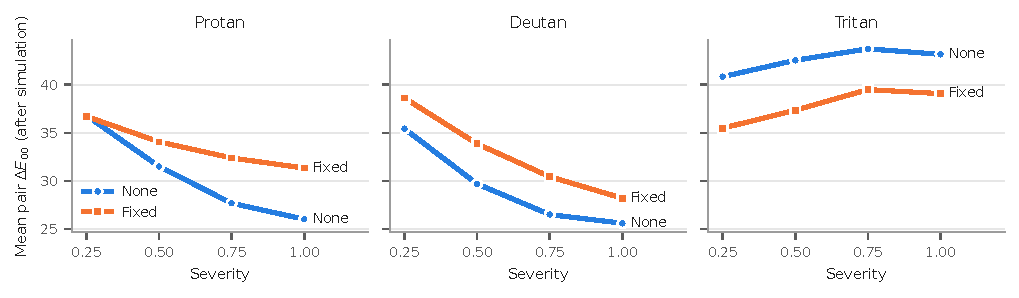
\includegraphics[width=\linewidth]{distinguishability_vs_severity}
  \caption{Mean pair distinguishability after CVD simulation as severity grows. Higher is
  better. Each line is one recoloring method.}
  \label{fig:severity}
\end{figure*}

\Cref{tab:recolor} and \cref{fig:severity} summarize the results. Without recoloring, pairs
lose distinguishability steadily as protan and deutan severity grows, falling to
\ResPairNoneProtanFull{} and \ResPairNoneDeutanFull{}~$\Delta E_{00}$ at full severity. The
fixed daltonization filter recovers part of that loss for red--green deficiencies:
\ResPairFixedProtanFull{} (protan) and \ResPairFixedDeutanFull{} (deutan) at full severity.
Across severities the deutan improvement is statistically reliable (median gain
\ResMedFixedDeutan~$\Delta E_{00}$, better on \ResImprovedFixedDeutan{} images,
$p_\mathrm{Holm}\ResPFixedDeutan$), while the protan gain is not
($p_\mathrm{Holm}\ResPFixedProtan$) because the filter changes little at low severity
(\cref{tab:paired}). For tritan the fixed filter is harmful: distinguishability drops from
\ResPairNoneTritan{} to \ResPairFixedTritan{}~$\Delta E_{00}$ (median
\ResMedFixedTritan, $p_\mathrm{Holm}\ResPFixedTritan$). A likely reason is that the Machado
tritan model shifts colors only slightly, so pairs remain well separated without help, while
the filter still moves them. The price of recoloring is a naturalness change of
\ResNatFixedDeutan--\ResNatFixedProtan~$\Delta E_{00}$ per pixel (\cref{fig:naturalness}).

\begin{table}[t]
  \centering
  \footnotesize
  \begin{tabular}{@{}llrrrr@{}}
\toprule
Method & Type & $n$ & Median $\Delta$ & Improved & $p_\mathrm{Holm}$ \\
\midrule
Fixed & Protan & 51 & +1.6 & 28/51 & 0.111 \\
Fixed & Deutan & 51 & +4.9 & 35/51 & 0.009 \\
Fixed & Tritan & 51 & -4.7 & 11/51 & \ensuremath{<}0.001 \\
\bottomrule
\end{tabular}

  \caption{Each method against no recoloring: per-image pair distinguishability (averaged
  over severities), two-sided Wilcoxon signed-rank tests with Holm correction. \emph{Improved}:
  images where the method raised distinguishability.}
  \label{tab:paired}
\end{table}

\begin{figure}[t]
  \centering
  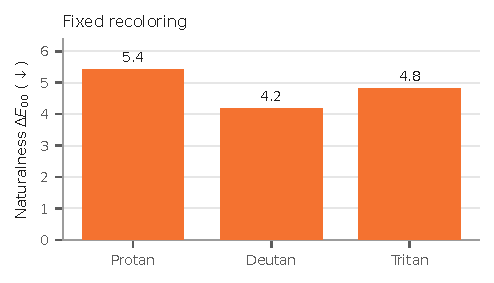
\includegraphics[width=\linewidth]{naturalness}
  \caption{Naturalness cost: mean per-pixel $\Delta E_{00}$ between the original and the
  recolored image for normal vision (lower is better). No recoloring is 0 by definition.}
  \label{fig:naturalness}
\end{figure}

\paragraph{By category.}
Gains depend on content (\cref{tab:category}). At full severity, averaged over CVD types,
natural scenes gain the most (\ResCatNoneNatural{} to \ResCatFixedNatural~$\Delta E_{00}$),
where red flowers and fruit sit on green foliage (\cref{fig:example}). Charts get slightly
worse (\ResCatNoneCharts{} to \ResCatFixedCharts), suggesting that when a chart's palette already
stays separable, the filter can push some series toward each other.

\begin{table}[t]
  \centering
  \footnotesize
  \begin{tabular}{@{}lcc@{}}
\toprule
Category & None & Fixed \\
\midrule
Charts & 27.9 & 25.2 \\
Maps & 33.4 & 33.1 \\
Traffic & 39.3 & 41.8 \\
Food & 29.5 & 31.4 \\
Coded items & 33.5 & 34.2 \\
Natural & 26.5 & 32.6 \\
\bottomrule
\end{tabular}

  \caption{Pair distinguishability ($\Delta E_{00}$) at severity 1.0 by category, averaged
  over CVD types.}
  \label{tab:category}
\end{table}

\begin{figure*}[t]
  \centering
  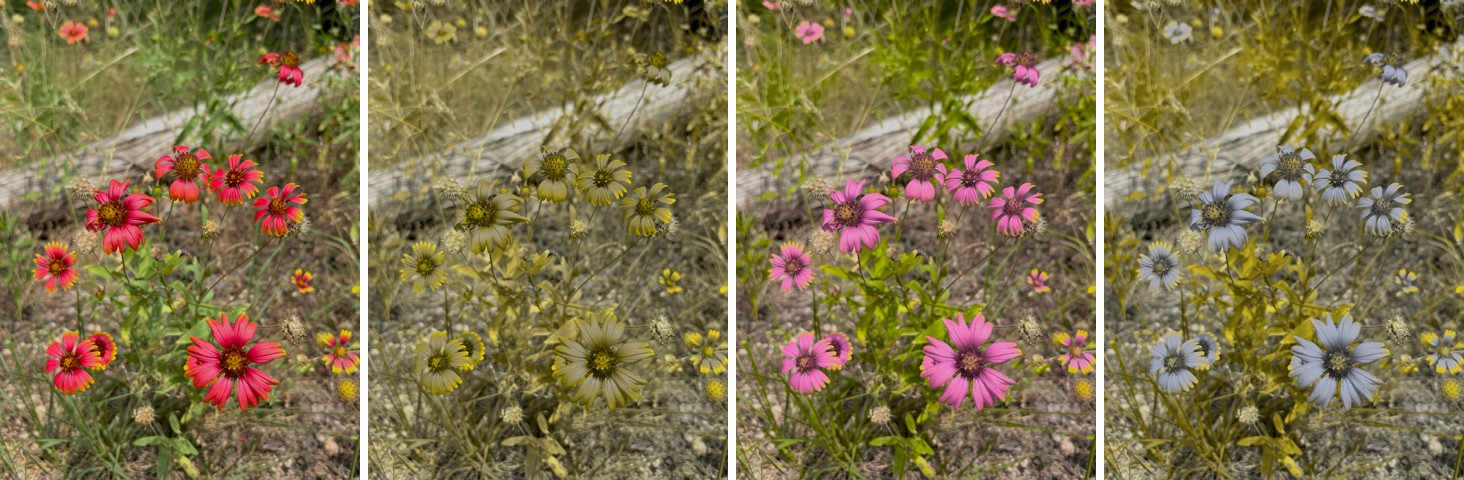
\includegraphics[width=\linewidth]{example.jpg}
  \caption{A team photograph (\ExampleImage). Left to right: original; deutan simulation
  (severity 1.0); fixed recoloring; deutan simulation of the recolored image. The red flowers
  that merge with the foliage under simulation become separable after recoloring.}
  \label{fig:example}
\end{figure*}

\ifdefined\ResPairPersonalizedDeutan
\paragraph{Personalized recoloring.}
With parameters tuned per type and severity on the tune split, personalized daltonization
reaches \ResPairPersonalizedDeutan{} (deutan) and \ResPairPersonalizedProtan{} (protan)
mean pair $\Delta E_{00}$, against \ResPairFixedDeutan{} and \ResPairFixedProtan{} for the
fixed filter, at a naturalness cost of \ResNatPersonalizedDeutan{} (deutan).
\TODO{Aliza: interpret once personalized results are in.}
\else
\paragraph{Personalized and neural recoloring.}
\TODO{Personalized and neural results appear here automatically: re-run run\_eval and
report\_assets once each method is available.}
\fi

\paragraph{Limitations.}
Distinguishability is measured on simulated vision, not on observers. The pairs were chosen to
be clearly different for normal vision, so the share below the JND is close to zero for every
method, and the metric reflects how much separation survives rather than whether pairs become
indistinguishable. Region means ignore texture and spatial context, and a single JND for all
pairs ignores region size.

\subsection{User study}
\label{sec:study}
Participants played the color-match game of \cref{sec:app}: each trial shows a test image with
two outlined regions from our annotations and asks which one answers a prompt such as ``which
apple is red?''. Each image appears under one recoloring condition per participant, rotated
across participants. For every participant and condition we compute accuracy and the median
response time of correct trials, then compare conditions with paired Wilcoxon signed-rank
tests~\cite{wilcoxon1945}, Holm-corrected~\cite{holm1979}, reporting the matched-pairs
rank-biserial correlation $r$~\cite{kerby2014} as effect size.

Each log records the CVD profile \emph{applied in the game}, not a diagnosis: normal-vision
players are given a simulated deutan profile (\cref{sec:app}), so they see the recolored image
through the deutan simulation. Their results therefore describe recoloring as seen through
simulated deutan vision, not by people with CVD. We report a separate subgroup only for
participants whose screening found a CVD, taken from the screening results rather than from
the logs.

\begin{table}[t]
  \centering
  \footnotesize
  \begin{tabular}{@{}lrrr@{}}
\toprule
Condition & Participants & Accuracy (\%) & Median RT (s) \\
\midrule
\multicolumn{4}{c}{\emph{No study sessions logged yet.}} \\
\bottomrule
\end{tabular}

  \caption{Mini-game results per condition (mean $\pm$ SD across participants; median of
  per-participant median response times on correct trials).}
  \label{tab:study}
\end{table}

\ifnum\StudyParticipants>0
\Cref{tab:study} summarizes \StudyTrials{} trials from \StudyParticipants{} participants.
\StudySimulatedParticipants{} of them played with a simulated CVD profile and
\StudyCvdParticipants{} were found to have a CVD by screening\ifnum\StudyCvdParticipants=0{},
so no result here describes observers with CVD\fi.
\TODO{Aliza: interpret the comparisons in results/study\_comparisons.csv.}
\else
\TODO{Study sessions have not been run yet; \cref{tab:study} fills in automatically from the
logs in results/study/ when \texttt{scripts/analyze\_study.py} is re-run.}
\fi
